\begin{pastexam}[label={px:ntu-110-comm-dsa-17}]{臺大電信所 110 學年度（B）第 17 題}
（單選；每題 2 分，答錯不倒扣）

Consider the following undirected connected graph. What is the total weight of its maximum spanning tree?

\begin{center}
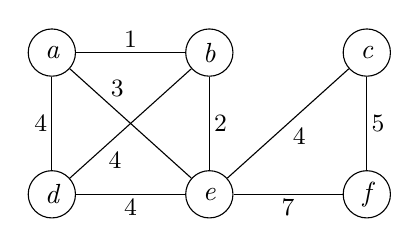
\begin{tikzpicture}[v/.style={circle,draw,inner sep=1pt,minimum size=6mm,font=\itshape},l/.style={inner sep=1.5pt,font=\small}]
\node[v] (a) at (0,1.8) {a}; \node[v] (b) at (2,1.8) {b}; \node[v] (c) at (4,1.8) {c};
\node[v] (d) at (0,0) {d}; \node[v] (e) at (2,0) {e}; \node[v] (f) at (4,0) {f};
\draw (a) -- node[l,above] {1} (b);
\draw (a) -- node[l,left] {4} (d);
\draw (a) -- node[l,pos=0.3,above right] {3} (e);
\draw (b) -- node[l,pos=0.72,below right] {4} (d);
\draw (b) -- node[l,right] {2} (e);
\draw (d) -- node[l,below] {4} (e);
\draw (e) -- node[l,below right] {4} (c);
\draw (c) -- node[l,right] {5} (f);
\draw (e) -- node[l,below] {7} (f);
\end{tikzpicture}
\end{center}

A.~23 \qquad B.~24 \qquad C.~25 \qquad D.~26
\end{pastexam}

\begin{pastsoln}
答案是 B（24）。

最大生成樹就是把 Kruskal 的排序反過來：邊由大到小考慮，兩端不在同一棵樹就加入（資結書第~24.2~節）。
正確性和最小生成樹一樣，因為把每條邊權改成 $-w$ 後，最大生成樹就是最小生成樹。

圖有 $6$ 個頂點，生成樹要 $5$ 條邊。 邊由大到小（同權重的順序不影響總權重）：
\begin{center}
\begin{tabular}{clll}
\toprule
邊 & 權重 & 動作 & 加入後的集合 \\
\midrule
$e$--$f$ & 7 & 加入 & $\{e, f\}$ \\
$c$--$f$ & 5 & 加入 & $\{c, e, f\}$ \\
$a$--$d$ & 4 & 加入 & $\{a, d\}$、$\{c, e, f\}$ \\
$b$--$d$ & 4 & 加入 & $\{a, b, d\}$、$\{c, e, f\}$ \\
$d$--$e$ & 4 & 加入 & $\{a, b, c, d, e, f\}$ \\
\bottomrule
\end{tabular}
\end{center}
加到第 $5$ 條邊就連通了。 之後的 $e$--$c$（4）、$a$--$e$（3）、$b$--$e$（2）、$a$--$b$（1）兩端都已
在同一集合，全部略過。 總權重 $7 + 5 + 4 + 4 + 4 = 24$，選 B。

檢查：權重 $4$ 的邊有四條（$a$--$d$、$b$--$d$、$d$--$e$、$e$--$c$），但 $c$ 已經由 $c$--$f$--$e$ 連上，
$e$--$c$ 會成環，所以四條只能用三條；7 和 5 一定會選（它們是各自割上的最大邊）。 不可能更大：$5$ 條邊
裡最大的兩條是 $7$、$5$，其餘三條至多各 $4$，上界正是 $24$。
\end{pastsoln}
